\documentclass{article}

\usepackage{wrapfig}
\usepackage{lmodern}
\usepackage[T1]{fontenc}
\usepackage[spanish]{babel}
\usepackage{mathtools}
\usepackage{graphicx}
\usepackage[utf8]{inputenc}


\title{TEMA 4 BASES DE DATOS}
\author{Antonio Muñoz Cubero}
\date{5 de Ocutbre de 2020} 


\begin{document}
\maketitle
\pagenumbering{roman}

\newpage

    \tableofcontents

\newpage
\section{Introducción}
El modelo entidad/relación es un modelo conceptual ya que es un modelo que permite captar la mayor parte de la semántica del mundo real.
Dentro de los modelos conceptuales el que mayor aceptación tiene es este que permite representar de forma gráfica una base de datos. El trabajo del 
consultor o analista informático consiste en tres pasos:
\begin{itemize}

    \item 1. Entender el modelo de negocio con detalle, comprendiendo las necesidades del cliente.
    \item 2. Plasmar el modelo de negocio mediante el diagrama entidad/relación.
    \item 3. A partir del esquema del paso anterior, hacer el diseño relacional de las escrituras de datos y los procedimientos para poder manejar.

\end{itemize}

\subsection{Historia}
El modelo entidad/relación también se le conoce como el modelo de CHEN, ya que, fue su creador en 1976. Este modelo pretende describir la estructura de 
una base de datos independientemente de lo físico. Era muy pobre en sus orígenes, pero se ha ido mejorando mucho con los años con los añadidos de otros 
autores, se basa en las entidades presentes en un problema y las relaciones que hay entre ellas.

\section{Estática del Modelo E-R}
Describe las entidades e interrelaciones (con sus atributos) que existen en el mundo real. También incluyen los dominios.

\subsection{Entidad}
Es una persona, lugar, cosa, concepto… real o abstracto que sea de interés para nuestro modelo. Aquel “ente” sobre el que queremos guardar información. 
Tendremos por un lado lo que será el tipo de entidad, genérico, y por otro lado la ocurrencia del tipo de entidad que será cada uno de los valores que toma.
Se representa mediante un rectángulo, con el nombre del tipo de entidad dentro.
\textit{Clases de tipo de entidad:}

\begin{itemize}
    \item Las \textbf{regulares o fuertes}, las ocurrencias del tipo de entidades existen por sí mismas.
    \item Las \textbf{débiles}, en estas las existencias de una ocurrencia depende de que existan una ocurrencia de otra entidad regular de la cual depende. 
    Si desaparece la ocurrencia de la regular, desaparece la de la débil. Se representa en un recuadro doble.
\end{itemize}

\subsection{Interrelación}
Se da la correspondencia-relación que hay entre las entidades. El tipo de interrelación será genérico entre dos o más tipos de entidades, y la ocurrencia de 
un tipo de interrelación será la vinculación concreta entre ocurrencias en tipos de entidades. Se representa con un rombo con el nombre de la relación dentro, 
y líneas que unen este rombo a las entidades que relaciona.
\\
Características de una \textbf{Interrelación}:

\begin{itemize}

    \item \textbf{Nombre}: \textit{se pone para identificar la interrelación y suele ser un verbo. No debe haber dos con el mismo nombre en la base de datos.}
    \item \textbf{Grado}: \textit{es el número de entidades que se relacionan, las hay de grado uno (unarias) que asocian una entidad consigo misma, de grado 
    dos (binarias) que asocian dos entidades. Son las más comunes y fáciles de manejar. Lo ideal es tener solo interrelaciones binarias. También las hay de 
    grado tres (ternarias) que asocian tres entidades, son más difíciles de encontrar y siempre que podamos las transformaremos en binarias, que normalmente 
    se puede hacer transformando la interrelación en entidad. Y así hasta grado N…}
    \item \textbf{Tipo de Correspondencia}: \textit{es el número máximo de ocurrencias de un tipo de entidad que intervienen por cada ocurrencia del otro tipo 
    de entidad de la relación. Los tipos de correspondencia son:}

    \begin{itemize}
        \item \textbf{1:1} \textit{para cada ocurrencia de un tipo de entidad puede existir solo una como máximo de la otra y viceversa.}
        \item \textbf{1:N} \textit{para cada ocurrencia de un tipo de entidad pueden existir varias de la otra y solo una a la inversa.}
        \item \textbf{N:M} \textit{pueden existir varias ocurrencias de la otra y viceversa.}
    \end{itemize}

\end{itemize}

Otra cosa importante que hay que decir, es que, entre dos tipos de entidad puede existir más de un tipo de interrelación.
\newpage
\subsection{Atributos}
Son cada una de las propiedades que tiene un tipo de entidad o de interrelación. Se dan los datos concretos que queremos guardar de cada entidad o interrelación. 
Por ejemplo: nombre, apellidos, teléfono o fecha de nacimiento de una persona.
\\
El conjunto de posibles valores que puede tomar un atributo es el dominio. Los atributos se representan gráficamente con un óvalo unido a la entidad o interrelación, 
y el nombre del atributo dentro. También puede hacerse poniendo el nombre del atributo al lado de un circulo que estará conectado a la entidad o interrelación.\\
De los atributos de las entidades se debe elegir uno o más que identifiquen univoca y mínimamente la ocurrencia de esa entidad (se dan los campos claves). 
En cada entidad debe existir el atributo identificador principal (AIP) (clave principal); y si hay más de uno existirá también el atributo identificador candidato 
(AIC) (clave alternativa). Si hay más de uno se elegirá uno como principal (normalmente el de mayor uso) y los otros serán alternativos.
\\
\begin{wrapfigure}{r}{0.5\textwidth}
    \centering
    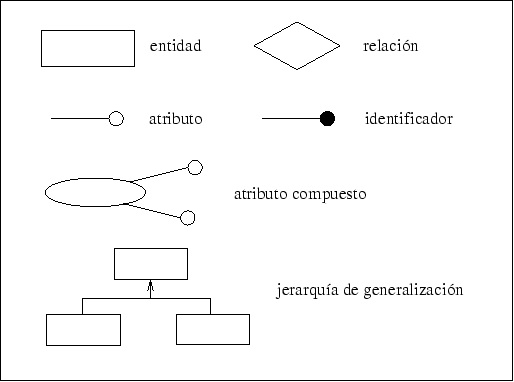
\includegraphics[width=0.5\textwidth]{entidad.jpg}
\end{wrapfigure}
\\
Para representar las partes principales lo haremos mediante un círculo relleno y las claves alternativas mediante un circulo mitad relleno y mitad vacío.
También pueden aparecer en las entidades las claves ajenas o foráneas que serán un atributo o conjunto de estos que existen en una entidad y que forman parte de la clave 
primaria en otra entidad con la que se relacionan. Estas claves no es necesario ponerlas en el esquema E-R, se quedarán en la entidad que correspondan y posteriormente al 
desarrollar el esquema relacional se propagaran y formaran la clave ajena (yo en algunos esquemas las pondré con línea discontinua unidas a la entidad donde son claves ajenas).
\\
\newpage
\textbf{Atributos en las interrelaciones} son atributos de interés para el modelo y que no corresponden de forma exclusiva a ninguna de las entidades que se interrelacionan, 
teniendo que ver con ambas, pero sin llegar a ser de ninguna en particular. Debido a esto se sitúan unidas al rombo de la interrelación.
\\
\textbf{Otros tipos de atributos} a la hora de diseñar un esquema E-R nos podemos encontrar con algunos atributos un poco especiales, que nos podrían plantear dudas sobre su 
representación. Vamos a comentar algunos de ellos, indicando posibles soluciones.

\begin{itemize}
    \item \textbf{Atributos atómicos o compuestos}: \textit{son datos simples como, por ejemplo, edad, nota, talla… mientas que los compuestos son los que a su vez se pueden dividir en varios 
    atómicos como, por ejemplo, dirección, que se podría dividir en calle, numero, piso, localidad… existen varias formas de representar los atributos compuestos, pero nosotros 
    lo haremos como los atómicos a no ser que nos digan expresamente que hay que guardarlos por separado.}
    \item \textbf{Atributos monovaluados y multivaluados:} \textit{los primeros serían, por ejemplo, edad, que tiene un solo valor y los multivaluados seria, por ejemplo, teléfonos, que podrían 
    tener más de uno. En el caso de los segundos podemos repetir el atributo añadiéndole un número, o mantener solo teléfonos, incluyendo a todos. Nosotros optaremos por la segunda opción a no 
    ser que nos digan lo contrario.}
    \item \textbf{Atributos derivados}: \textit{son aquellos que se pueden obtener a partir de otro atributo del que derivan o a partir de las interrelaciones. Por ejemplo, edad, que se puede 
    obtener a partir de la fecha de nacimiento y de la fecha del sistema, además la edad es un dato que varía con el tiempo mientras que la fecha de nacimiento es fija. Por tanto, es mejor guardar 
    la fecha de nacimiento que la edad y esto lo haremos siempre así a no ser que nos indiquen expresamente lo contrario.}
\end{itemize}

\subsection{Restricciones}
Puede haber dos tipos:
\\
\begin{itemize}
    \item \textbf{Restricciones semánticas o de integridad}: \textit{Restringen los valores válidos de ciertos atributos o limitan las correspondencias. Por ejemplo, del primero sería, el número 
    de páginas de un libro debe ser un numero entero, sin decimales, y además debe ser positivo. Del segundo, podría ser, que todo ejemplar de libro corresponde siempre a un único libro.}
    \item \textbf{Restricciones inherentes}: \textit{Son las propias de cada modelo, en el caso del modelo E-R, las únicas restricciones inherentes que tienen son: toda entidad debe de tener una 
    clave principal, las interrelaciones tienen que ser entre entidades, no entre una entidad y una interrelación, todas las entidades deben estar interrelaciones de forma directa o indirecta.}
\end{itemize}

\section{Cardinalidad de un tipo de entidad}
Cardinalidad máxima y mínima de los tipos de entidad implicados en una interrelación serán el número máximo y mínimo de ocurrencias de un tipo de entidad que pueden estar interrelacionados con una 
ocurrencia de la otra. Serán del tipo (0,1), (0,N), (1,1), (1,N), y se pondrá esa etiqueta según corresponda en la línea que une la entidad con el rombo de la interrelación Una interrelación no 
tendrá una sola cardinalidad, sino que tendrá una a cada una de sus lados.
\\
\textbf{La lectura de la cardinalidad se hace en este orden:}\\
\textit{1º [entidad] -> 2º [relación que hay] -> 3º[cardinalidad 2º entidad].}
\\
En el modelo E-R el tipo de correspondencia coincide con las cardinalidades máximas de los 2 tipos de entidades, así que solo pondremos las cardinalidades, ya que aportan más información y sería 
redundante poner ambas
\\
\\
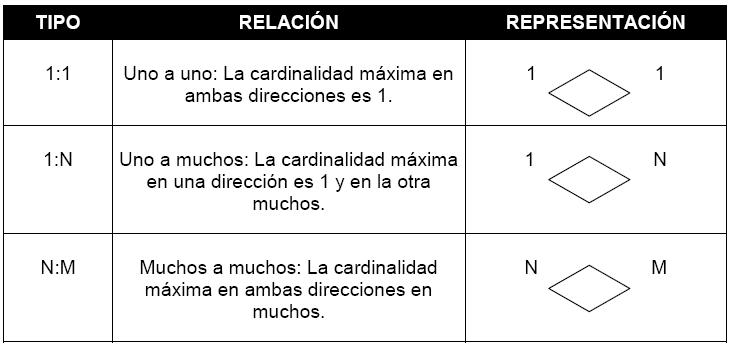
\includegraphics[width=1\linewidth]{dibujo.jpg}

\newpage
\subsection{Tipos De Interrelación}
\textbf{Fuertes o Regulares} asocian dos entidades regulares.
\textbf{Débiles} Asocian una entidad débil con otra Regular de la que depende. Estas exigen que al lado de la entidad Regular la cardinalidad sea siempre (1,1). Dos entidades débiles no pueden estar 
relacionadas.
\\
Dentro de la entidades débiles encontramos dependencia en \textbf{existencia} y en \textbf{identificación}.
\begin{itemize}
    \item \textbf{Dependencia en existencia:} \textit{en estas las ocurrencias del tipo de entidad débil no pueden existir sin la ocurrencias del tipo de entidad regular de la que depende. Se indican 
    mediante una \textbf{EX} en el rombo.}
    \item \textbf{Depende de identificación:} \textit{ademas de la dependencia de existencia, la entidad débil necesita de la clave de la regular
    para identificarse. se reperesenta mediante las letras \textbf{ID} en el rombo.}
\end{itemize}
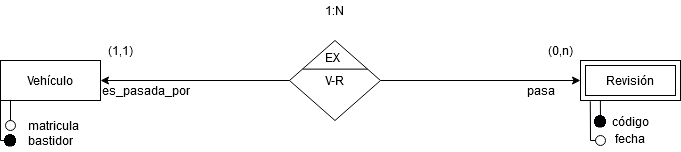
\includegraphics[width=1\linewidth]{existencia.png}
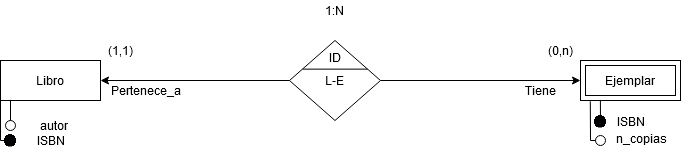
\includegraphics[width=1\linewidth]{identificacion.png}

\end{document}